\chapter{Conception de la solution}
\label{Conception de la solution}



Dans cette partie, nous allons commencer d’abord par le prototype de notre application. Ensuite, nous allons se concentrer sur la  vue architecturale du projet.Finalement, nous allons détailler la conception en présentant les
diagrammes de séquence et les diagrammes de classe. Ces diagrammes permettent de visualiser les différentes étapes du processus et la structure du système.

\pagebreak
\section{Prototypage}

Le prototypage est une étape importante dans le processus de développement de notre application. Il permet de créer une version préliminaire de
 l'application pour tester ces fonctionnalités, recueillir des retours utilisateurs, et identifier d'éventuelles améliorations avant de passer à la phase de développement complète.

 Dans cette section, nous décrirons les étapes de création du prototype

\subsection{Choix de l'outil}

\begin{figure}[H]
    \centering
    
\includegraphics[scale=0.05]{Logos/Figma.png}
    \caption{Logo Figma}
\end{figure} 

Figma est une plateforme collaborative pour éditer des graphiques vectoriels et faire du prototypage. Elle permet de concevoir des design systems pour faciliter la création de sites web et d’applications mobiles. C’est une solution à destination des UI et UX designers et des développeurs. L’interface propose de nombreuses fonctionnalités :

\begin{itemize}
    \item[$\bullet$] \textbf{Design:} avec des outils de conception pour le web, des fonctions de mise en page automatique, des plugins pour réduire les tâches répétitives.
    \item[$\bullet$] \textbf{Prototypage:} pour tester les concepts très tôt en cours de design.
    \item[$\bullet$] \textbf{Design system:} pour concevoir des design cohérents avec des bibliothèques mises à jour en permanence.
    \item[$\bullet$] \textbf{Collaboration:} pour travailler à plusieurs et en même temps sur un projet, revenir sur une version antérieure si nécessaire ou encore afficher le travail d’un seul collaborateur par exemple.
\end{itemize}

\subsection{Interface}

\subsubsection{Espace apprenant}

\begin{figure}[H]
    \centering
    \begin{minipage}{0.45\textwidth}
        \centering
        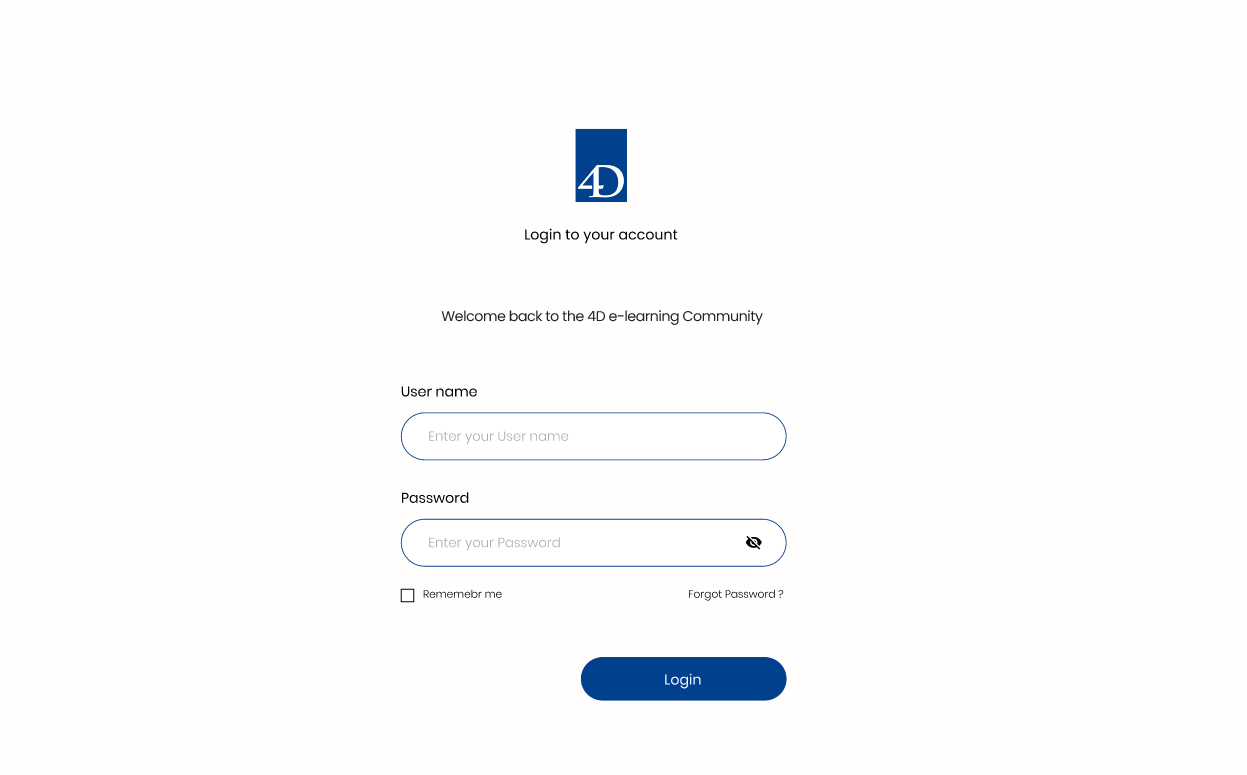
\includegraphics[width=\textwidth]{Figures/login.PNG}
        \caption{Figma: Page Login}
    \end{minipage}
    \hfill
    \begin{minipage}{0.45\textwidth}
        \centering
        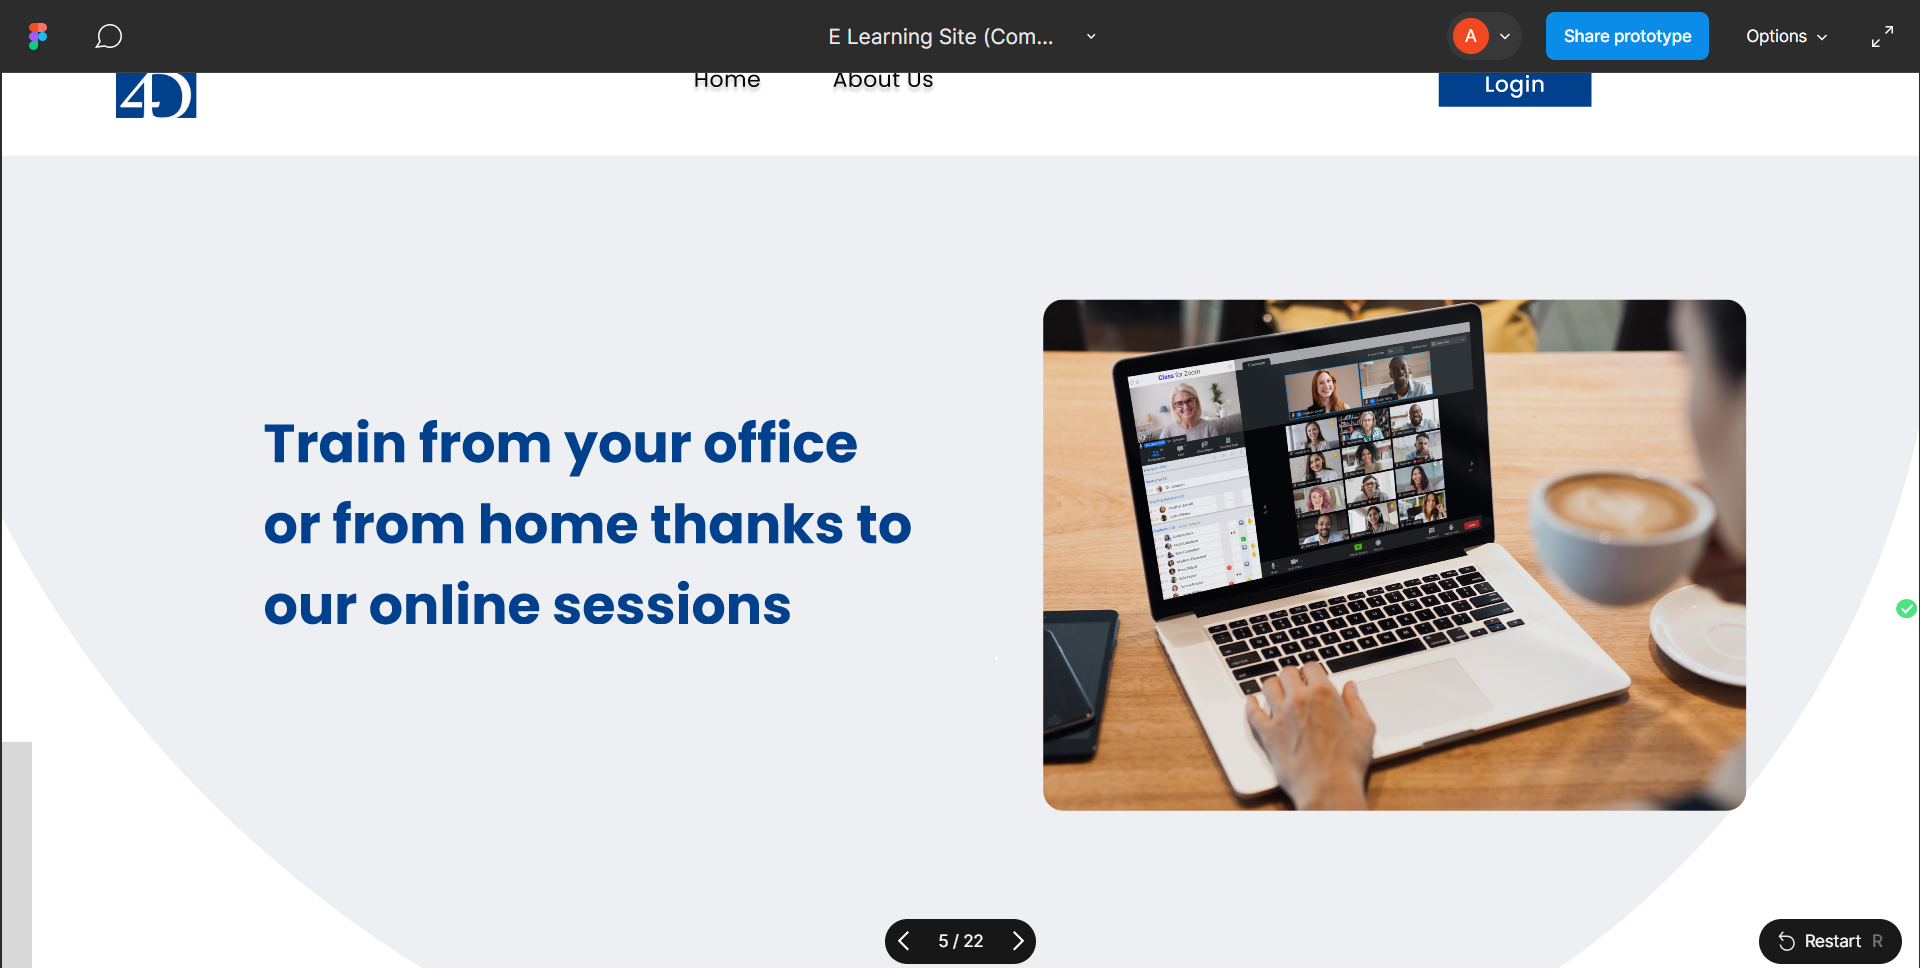
\includegraphics[width=\textwidth]{Figures/home.PNG}
        \caption{Figma: Page Home}
    \end{minipage}
\end{figure}

\begin{figure}[H]
    \centering
    \begin{minipage}{0.45\textwidth}
        \centering
        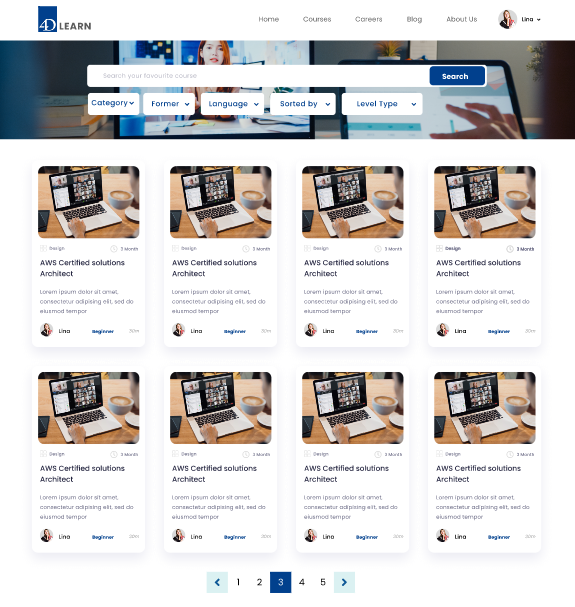
\includegraphics[width=\textwidth]{Figures/explorer.PNG}
        \caption{Figma: Page des Formations}

    \end{minipage}
    \hfill
    \begin{minipage}{0.45\textwidth}
        \centering
        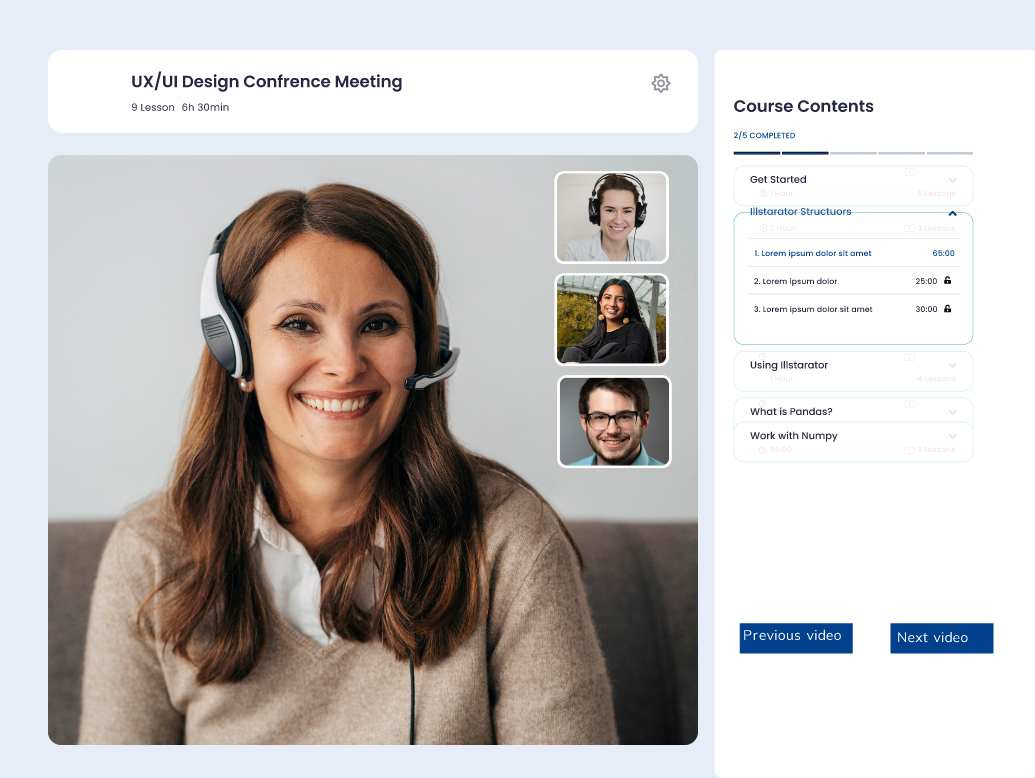
\includegraphics[width=\textwidth]{Figures/watchVideo.PNG}
        \caption{Figma: Page Suivre Formation }
        
    \end{minipage}
\end{figure}


\begin{figure}[H]
    \centering
    \begin{minipage}{0.45\textwidth}
        \centering
        
\includegraphics[width=\textwidth]{Figures/overview.PNG}
        \caption{Figma: Page Overview}
    \end{minipage}
    \hfill
    \begin{minipage}{0.45\textwidth}
        \centering
        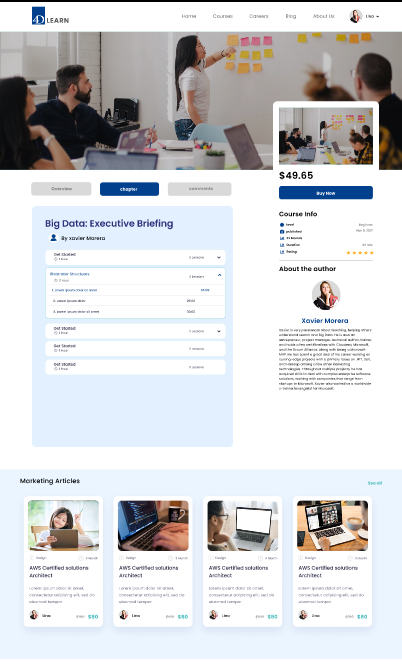
\includegraphics[width=\textwidth]{Figures/Chapter.PNG}
        \caption{Figma: Page des Chapitres }
    \end{minipage}
    
\end{figure}

\begin{figure}[H]
    \centering
    \begin{minipage}{0.45\textwidth}
        \centering
        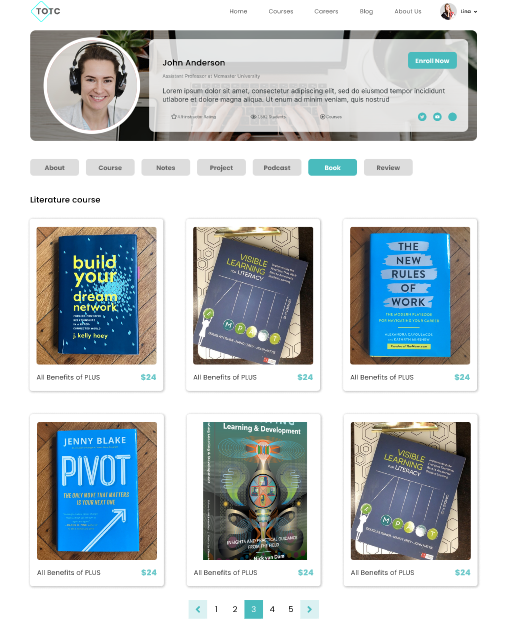
\includegraphics[width=\textwidth]{Figures/AuthorDetails.PNG}
        \caption{Figma: Page Détails d'un Formateur}
    \end{minipage}
    \hfill
    \begin{minipage}{0.45\textwidth}
        \centering
        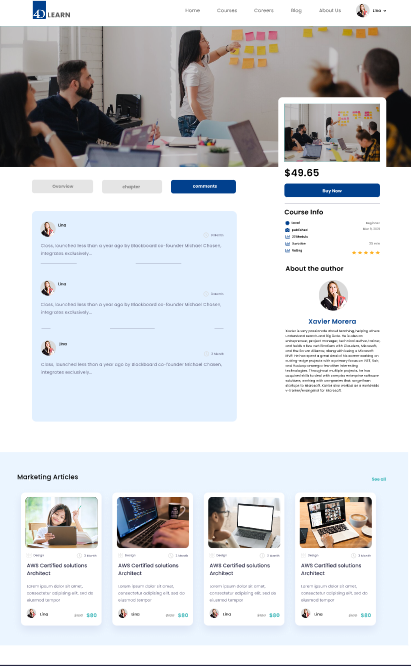
\includegraphics[width=\textwidth]{Figures/comment.PNG}
        \caption{Figma: Page des Chapitres}
    \end{minipage}
    
\end{figure}

\subsubsection{Espace administrateur}

\begin{figure}[H]
    \centering
    \begin{minipage}{0.45\textwidth}
        \centering
        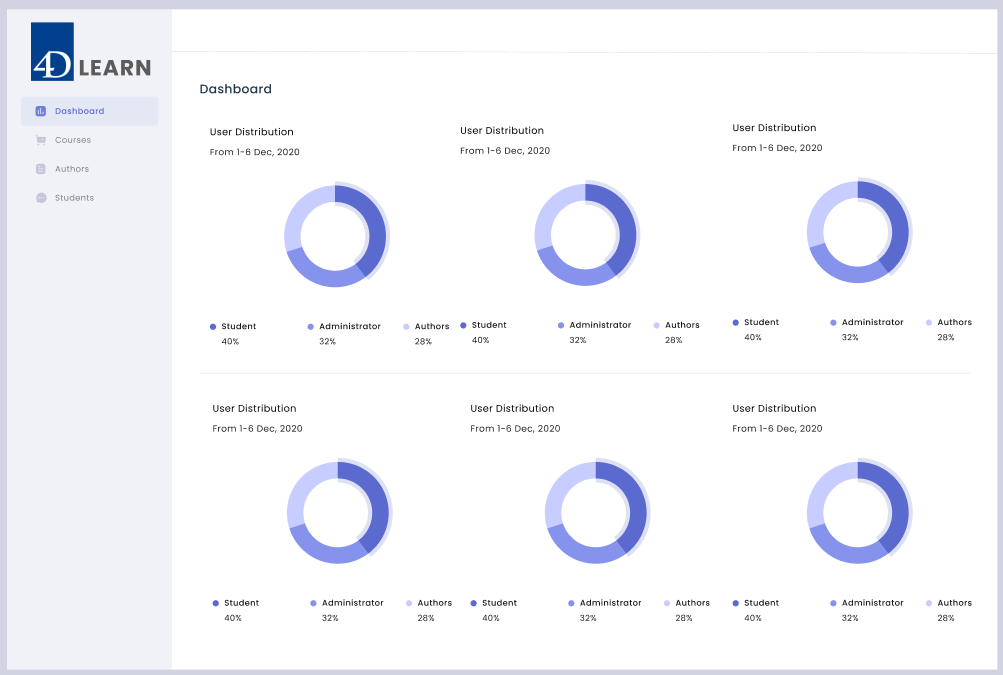
\includegraphics[width=\textwidth]{Figures/figmaDashoboard.PNG}
        \caption{Figma: Page Tableau De Board}
    \end{minipage}
    \hfill
    \begin{minipage}{0.45\textwidth}
        \centering
        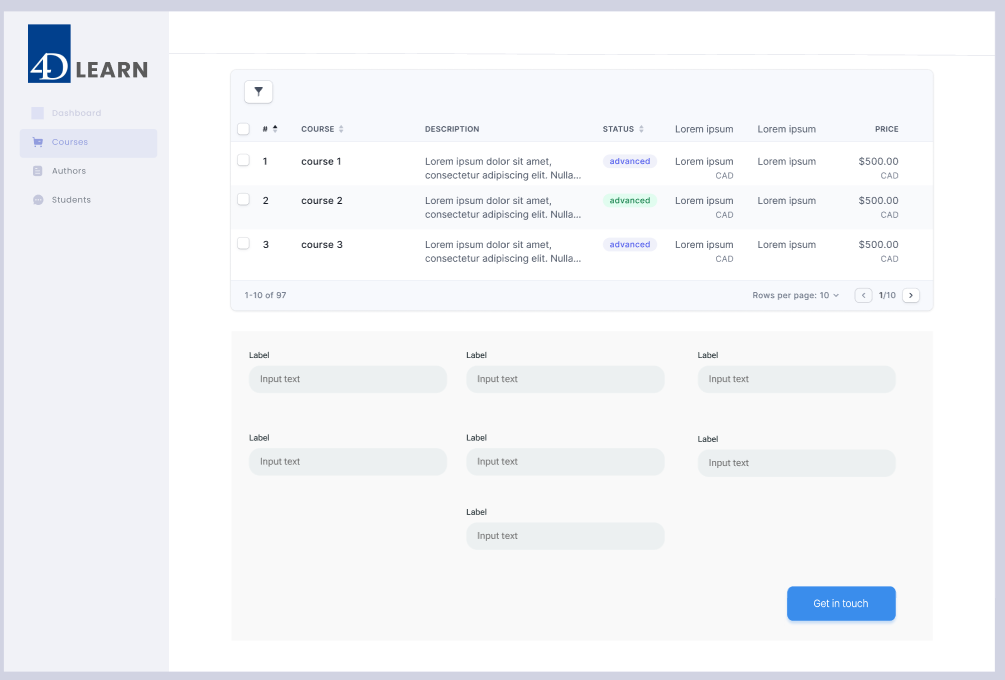
\includegraphics[width=\textwidth]{Figures/addCourseDashboard.png}
        \caption{Figma: Page D'ajout De Formation}
    \end{minipage}
    
\end{figure}

\section{Architecture de l’application}

\subsection{Architecture physique}

Nous avons opté pour l’architecture client/serveur multi-tiers. En effet, l’accès à l’application exige le passage à
travers des requêtes HTTP afin de récupérer et de déposer des versions dans le dépôt
central. De plus, la gestion de la base de données du système doit être centralisée et délocalisée de l’endroit de la couche métier, ce qui aide à garder une aisance de maintenance.
Et enfin, il faut que l’application soit distribuée sur plusieurs serveurs et chaque serveur
s’occupe d’une tâche. En effet, grâce au partage des tâches entre les différents serveurs,
nous pourrons garantir une grande souplesse, des bonnes performances et un temps de
réponse réduit. La figure suivante illustre l’architecture physique que nous avons :

\begin{figure}[H]
    \centering
    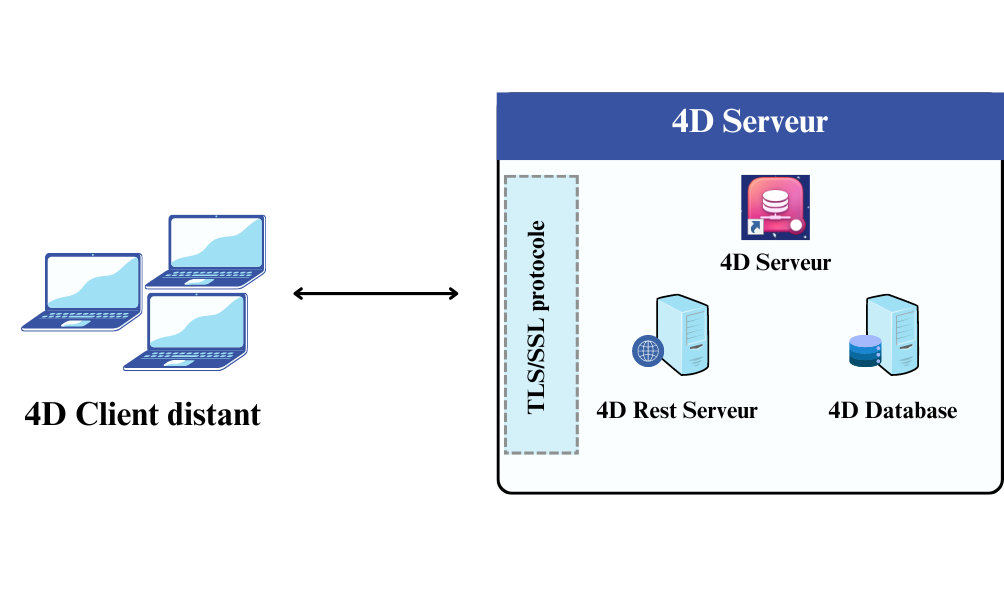
\includegraphics[width=15cm]{Figures/architecturePhysique.png}
    \caption{Architecture physique de système.}
\end{figure}

Cette architecture se compose principalement des éléments suivants :

\begin{itemize}
    \item[$\bullet$] \textbf{Serveur REST} : Un serveur web qui suit les principes de l'architecture REST et expose des ressources via des URI, permettant aux clients d'effectuer des opérations standardisées sur ces ressources pour accéder aux données et fonctionnalités du serveur.
    \item[$\bullet$] \textbf{Serveur 4D} : Ce serveur contient la couche métier de notre application.
    \item[$\bullet$] \textbf{Serveur de base de données} : Ce serveur se charge de la gestion du stockage des données.
    \item[$\bullet$] \textbf{Couche réseau} : Le protocole TLS sécurise les connexions client/serveur en cryptant les données échangées, permettant ainsi de renforcer la sécurité de notre application 4D Server.
\end{itemize}

\subsection{Architecture logique}

Dans notre architecture, nous avons utilisé le principe
de « Couche » pour séparer au maximum les différents types de traitement de l’application. L’environnement de travail n’est pas dépendant à une technologie spécifique.
Pour cette raison, nous avons utilisé plusieurs technologies afin de développer une solution multicouches  qui s’intègre parfaitement. La figure suivante
illustre l’architecture logicielle proposée pour le système développé, en présentant quatre
couches: couche présentation, couche controlleur, couche métier qui s’occupe des différents traitements
et couche accès aux données.


\begin{figure}[H]
    \centering
    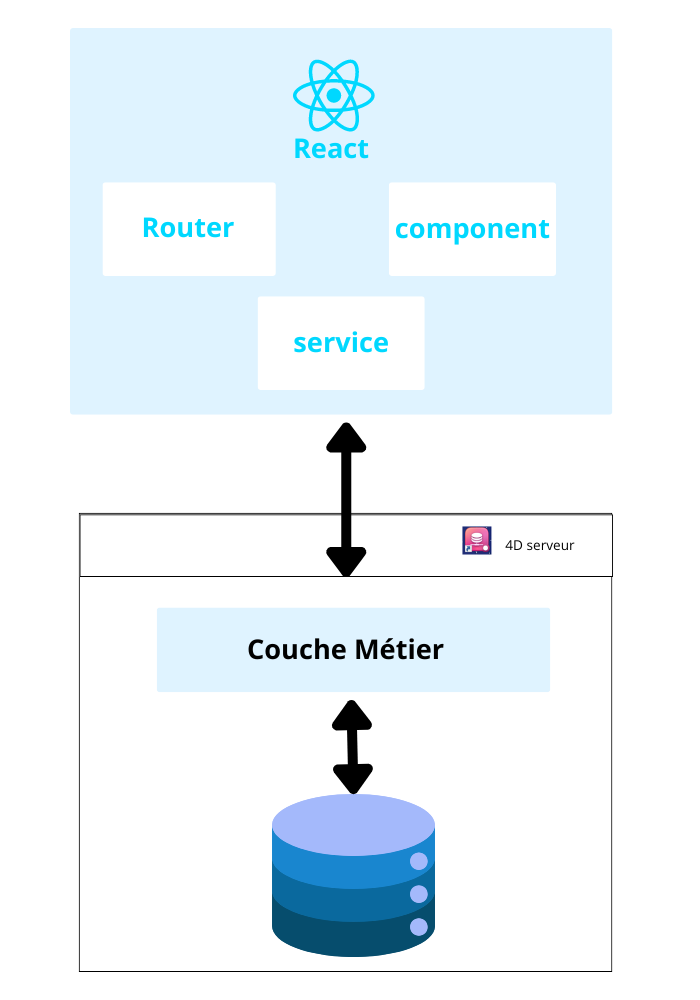
\includegraphics[width=9cm]{Figures/architectureLogique.png}
    \caption{Architecture logique de système.}
\end{figure}

Au niveau 4D Server, notre développement s’est concentré principalement sur la couche
métier. En effet, 4D Server offre un environnement de développement qui simplifie considérablement la création d’applications. Les autres couches, telles que la couche d’accès
aux données et la couche controlleur, sont déjà implémentées et intégrées dans 4D.Ainsi, les développeurs peuvent se concentrer sur la logique métier de leurs applications
sans avoir à se soucier des détails techniques des autres couches. Cette approche permet
un développement rapide et efficace, tout en offrant des fonctionnalités avancées pour
répondre aux besoins spécifiques des projets.

Aussi, nous avons travaillé avec ORDA (Object Relational Data Access), qui est une technologie spécifique qui facilite
l’accès à une base de données relationnelle en tant qu’objets. Elle permet de manipuler les
données de la base de données à l’aide d’un langage de programmation orienté objet ou
d’interfaces utilisateur spécifiques. ORDA simplifie l’interaction avec la base de données
en fournissant des abstractions supplémentaires et en masquant certaines complexités liées
aux requêtes SQL.

ORDA nous permet de créer des fonctions de classe de haut niveau au-dessus du modèle de données. Cela nous permet d'écrire du code orienté métier et de le «publier» comme une API. Le datastore, les dataclasses, les entity selections et les entités sont tous disponibles en tant qu'objets de classe pouvant contenir des fonctions.

\begin{figure}[H]
    \centering
    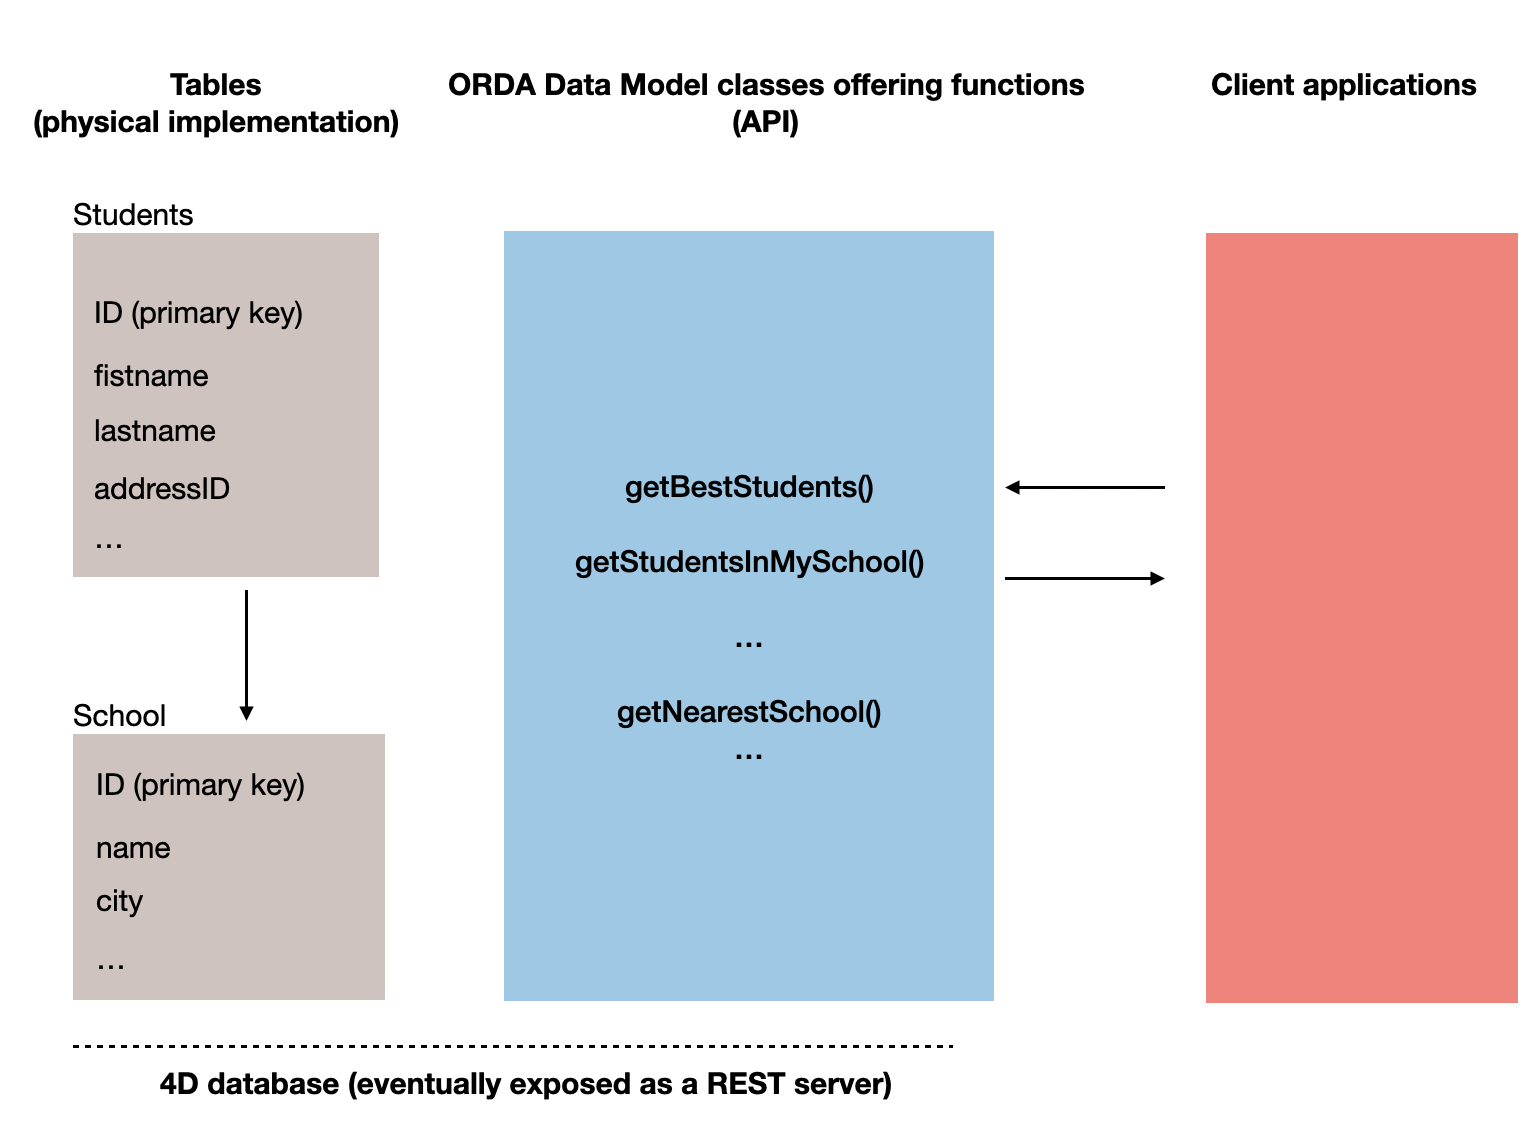
\includegraphics[width=15cm]{Figures/orda.png}
    \caption{Orda Data Model Class}
\end{figure}

Grâce à 4D, les développeurs peuvent se concentrer sur l’essentiel et créer des applications puissantes et performantes en toute simplicité.


\section{Conception Détaillée}

\subsection{Diagramme de Classe}
Le diagramme de classe est l’un des diagrammes statiques d’UML. Il permet de décrire
la structure d’un système informatique tout en montrant les différentes classes, leurs
attributs, leurs méthodes ainsi que les relations entre eux.

\begin{figure}[H]
    \centering
    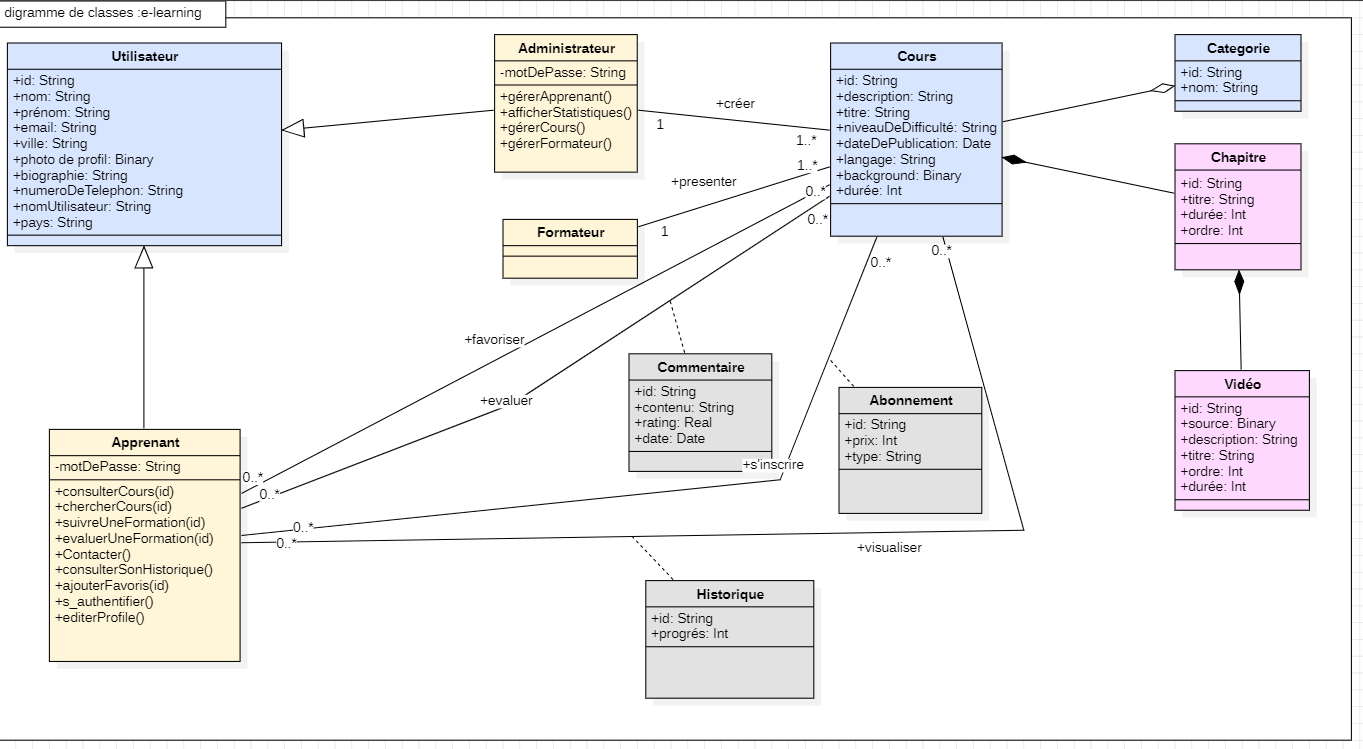
\includegraphics[width=19cm]{Figures/diagramme de classe.PNG}
    \caption{Diagramme de Classe}
\end{figure}

\subsection{Diagramme de séquence détaillé}

\subsubsection*{Diagramme de séquence de l'authentification}

Dans ce diagramme, nous avons essayé de montrer de manière plus détaillée comment un utilisateur peut s'identifier sur notre plateforme.

\begin{figure}[H]
    \centering
    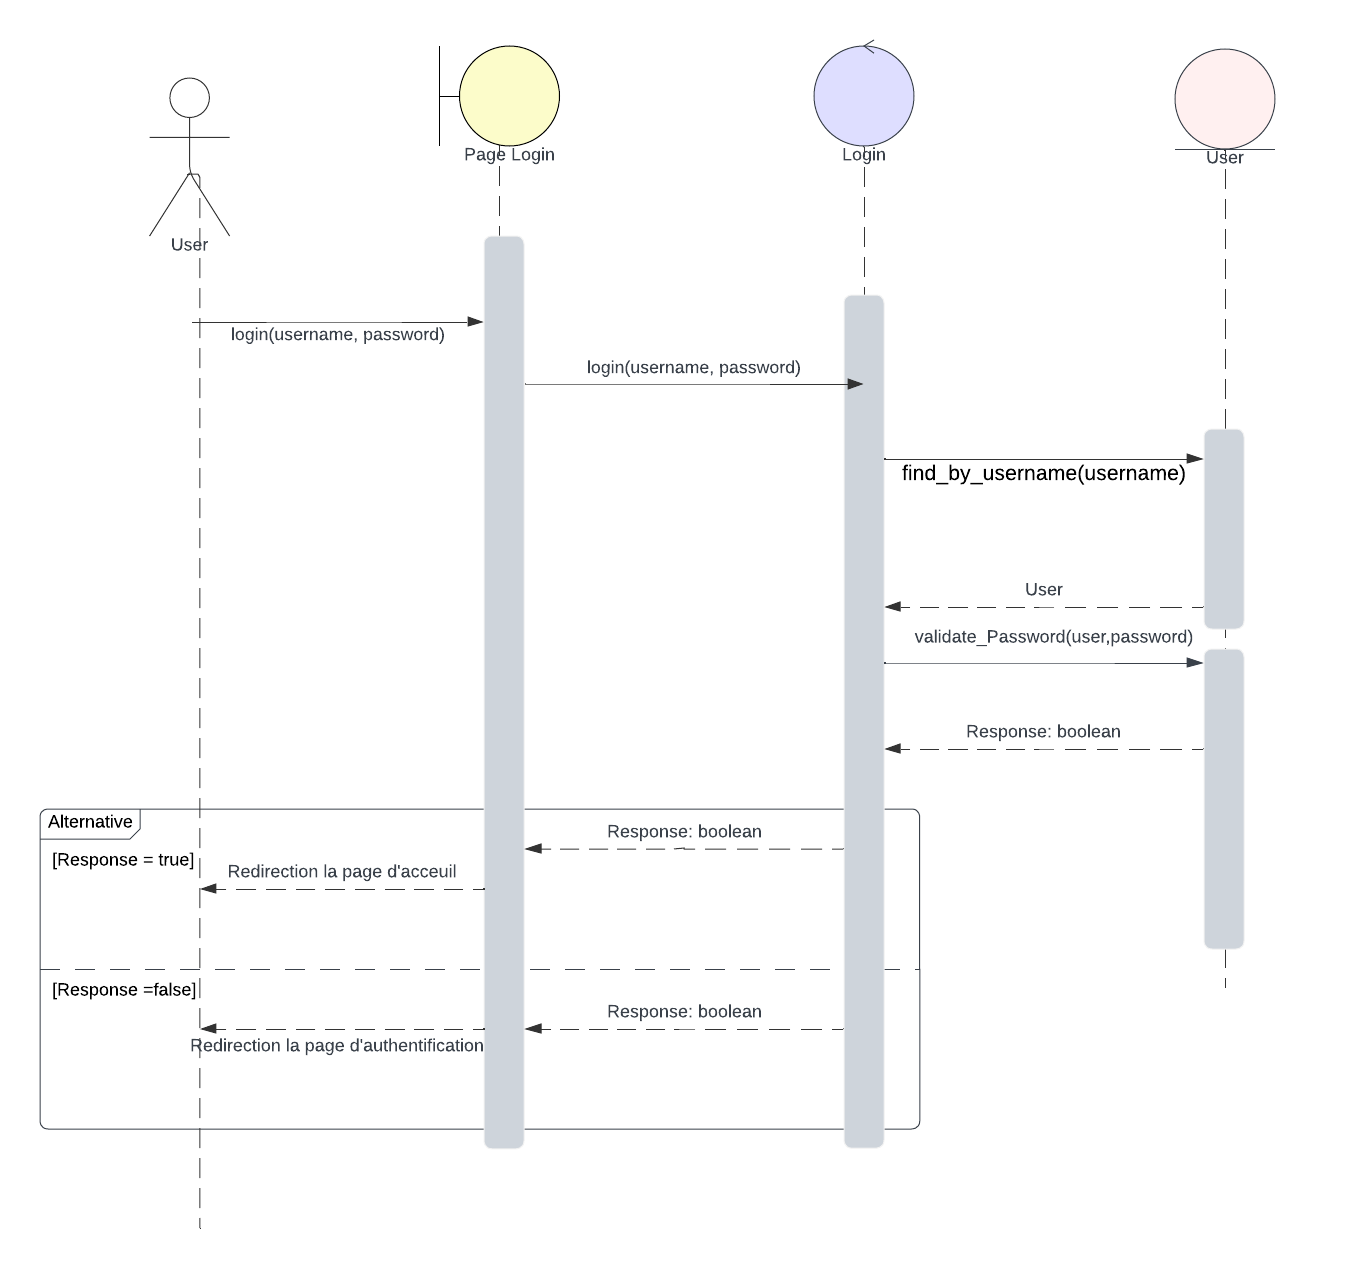
\includegraphics[width=19cm]{Figures/authdetaille.png}
    \caption{Diagramme de séquence détaillé de l'authentification}
\end{figure}

\subsubsection*{Diagramme de séquence d’ajouter une formation}

Ce diagramme montre comment le système ajoute une formation. D'abord, après avoir cliqué sur le bouton "Add Course", le système essaie d'abord d'enregistrer les informations de la formation. Ensuite, grâce à l'ID de la formation, on peut ajouter les chapitres liés à cette formation, ainsi que les vidéos. Tout cela se fait de manière transactionnelle pour s'assurer que le cours est ajouté correctement. 

\begin{figure}[H]
    \centering
    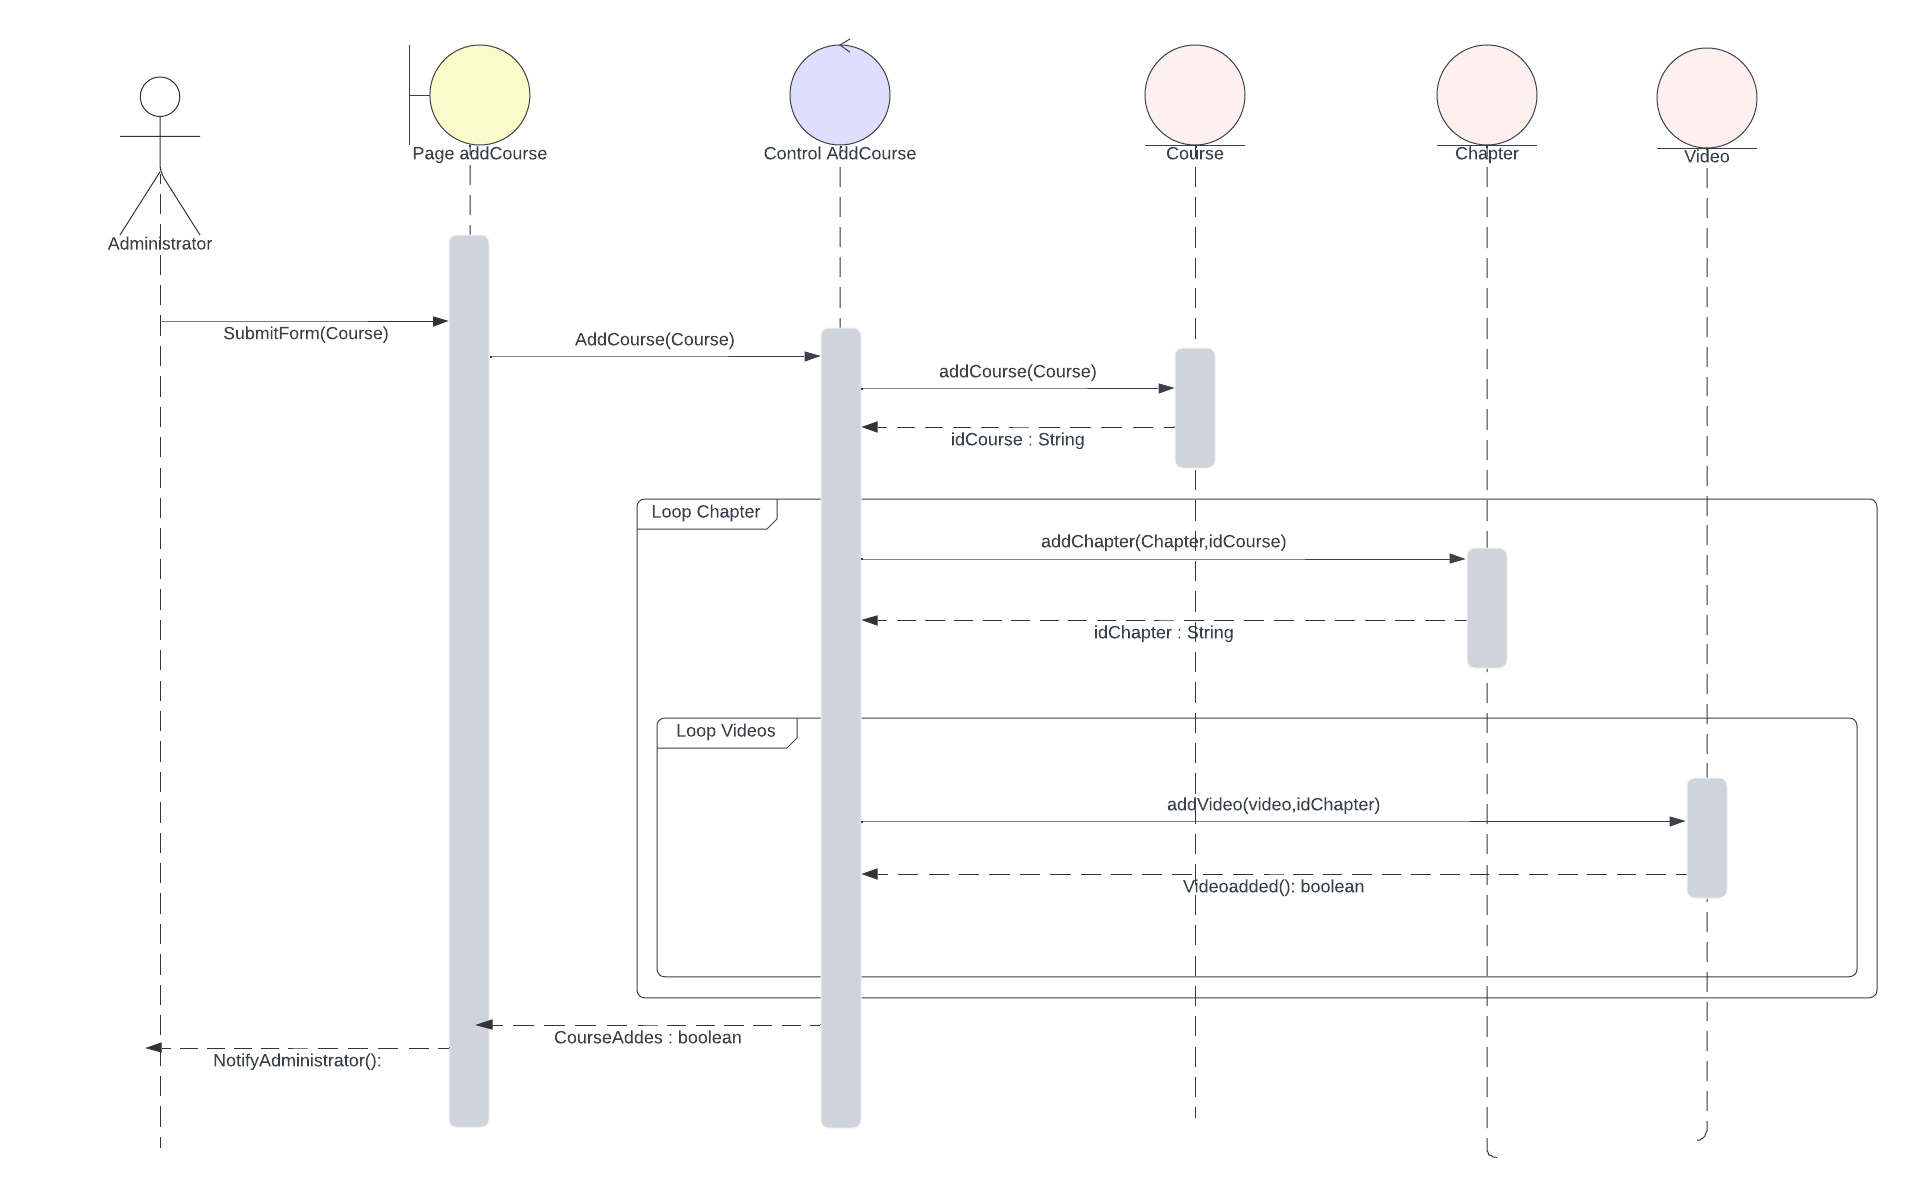
\includegraphics[width=19cm]{Figures/addcourseSequence.png}
    \caption{Diagramme de séquence détaillé d’ajouter une formation}
\end{figure}
\newpage
\subsection*{Conclusion}
Au cours de ce chapitre, nous avons d'abord présenté le prototype de notre application. Ensuite, nous avons examiné les architectures utilisées ainsi que les diagrammes de classes et de séquences. Nous allons maintenant entamer la partie de l'implémentation et la validation de notre solution.
